\documentclass[border=3pt]{standalone}
% Preâmbulo compartilhado pelos diagramas TikZ da aula 13 (SLAM com EKF)
\usepackage[T1]{fontenc}
\usepackage[utf8]{inputenc}
\usepackage{lmodern}
\usepackage{amsmath}
\usepackage{xcolor}
\usepackage{tikz}
\usetikzlibrary{arrows.meta,angles,quotes,decorations.pathmorphing,decorations.pathreplacing,calc,
                positioning,shapes.geometric,shapes.misc,backgrounds,fit,
                math}

% Paleta (mesma dos SVGs originais)
\definecolor{dblue}{HTML}{2A5B8C}
\definecolor{dorange}{HTML}{B3541E}
\definecolor{dgreen}{HTML}{4A7C59}
\definecolor{dred}{HTML}{9C4B4B}
\definecolor{dcream}{HTML}{F4F1EA}
\definecolor{dshade}{HTML}{DDD7C9}

% Função gaussiana (não normalizada por padrão de escala visual)
\pgfmathdeclarefunction{gauss}{3}{%
  \pgfmathparse{1/(#3*sqrt(2*pi))*exp(-((#1-#2)^2)/(2*#3^2))}%
}

% Estilos comuns (prefixo d... para não colidir com chaves internas do pgf)
\tikzset{
  >={Stealth[length=2mm]},
  dguide/.style={gray!55, dashed, line width=0.4pt},
  daxis/.style={gray!60, line width=0.7pt, ->},
  dbody/.style={fill=black!3, draw=black!80, line width=1pt},
  dacc/.style={draw=dblue, line width=1pt},
  dlbl/.style={black!55, font=\small},
  dsub/.style={black!45, font=\footnotesize},
  dstate/.style={circle, draw=black!80, fill=dcream, line width=1pt,
                 minimum size=17mm, font=\large, inner sep=1pt},
  dobs/.style={circle, draw=black!80, fill=dshade, line width=1pt,
               minimum size=14mm, font=\large, inner sep=1pt},
  dbox/.style={rounded corners=2pt, draw=black!80, fill=dcream, line width=1pt,
               align=center, inner sep=6pt},
  dop/.style={circle, draw=black!80, fill=white, line width=1pt,
              minimum size=6mm, inner sep=0pt, font=\small},
  dtrans/.style={->, dblue, line width=1pt},
  dmeas/.style={->, dorange, line width=1pt},
  dcurve/.style={line width=1pt, dblue},
  dcurveb/.style={line width=1.4pt, dorange},
}

\begin{document}
\hyphenpenalty=10000 \exhyphenpenalty=10000 \tolerance=9999 \emergencystretch=3em
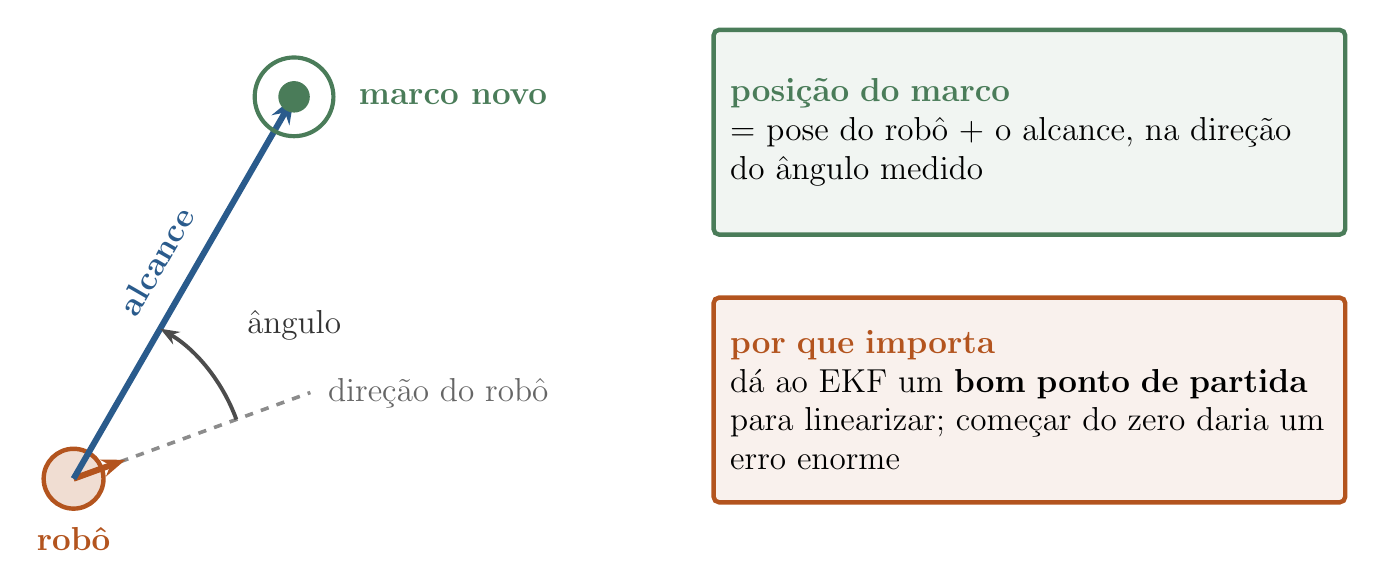
\begin{tikzpicture}[x=1cm,y=1cm]
\draw[black!45, dashed, line width=1.3pt] (2.5,1.6) -- ({2.5+3.2*cos(20)},{1.6+3.2*sin(20)});
\node[font=\large, black!60, anchor=west] at ({2.5+3.2*cos(20)+0.1},{1.6+3.2*sin(20)}) {direção do robô};
\draw[dorange, fill=dorange!20, line width=1.6pt] (2.5,1.6) circle (0.38);
\draw[dorange, line width=2.2pt, -{Stealth[length=3mm]}] (2.5,1.6) -- ({2.5+0.7*cos(20)},{1.6+0.7*sin(20)});
\node[font=\large\bfseries, dorange, anchor=north] at (2.5,1.1) {robô};
\draw[dblue, line width=2.2pt, -{Stealth[length=3.4mm]}] (2.5,1.6) -- ({2.5+5.6*cos(60)},{1.6+5.6*sin(60)});
\fill[dgreen] ({2.5+5.6*cos(60)},{1.6+5.6*sin(60)}) circle (0.2);
\draw[dgreen, line width=1.5pt] ({2.5+5.6*cos(60)},{1.6+5.6*sin(60)}) circle (0.5);
\node[font=\large\bfseries, dgreen, anchor=west] at ({2.5+5.6*cos(60)+0.7},{1.6+5.6*sin(60)}) {marco novo};
\draw[black!70, line width=1.4pt, -{Stealth[length=2.4mm]}] ({2.5+2.2*cos(20)},{1.6+2.2*sin(20)}) arc (20:60:2.2);
\node[font=\large, black!80] at (5.3,3.55) {ângulo};
\node[font=\large\bfseries, dblue, rotate=60] at ({2.5+2.9*cos(60)-0.4},{1.6+2.9*sin(60)+0.25}) {alcance};
\node[dbox, draw=dgreen, fill=dgreen!8, line width=1.6pt, text width=7.6cm, minimum height=2.6cm, font=\large, align=left, anchor=west] at (10.6,6.0) {\textbf{\textcolor{dgreen}{posição do marco}}\\ = pose do robô + o alcance, na direção do ângulo medido};
\node[dbox, draw=dorange, fill=dorange!8, line width=1.6pt, text width=7.6cm, minimum height=2.6cm, font=\large, align=left, anchor=west] at (10.6,2.6) {\textbf{\textcolor{dorange}{por que importa}}\\ dá ao EKF um \textbf{bom ponto de partida} para linearizar; começar do zero daria um erro enorme};
\end{tikzpicture}
\end{document}
